\section{Módulos}
Para a criação dos módulos de hardware, foram escolhidos componentes de \wiot{} comerciais, que possuem preços acessíveis, ampla documentação disponível e uma comunidade de desenvolvedores crescente.

A interconexão dos componentes, bem como a comunicação com o mundo externo pela Internet é intermediada por um servidor local, instalado e disponível na plataforma Raspberry Pi, rodando um sistema operacional Linux (Raspbian, baseado em Debian) e que dispõe da interface de hardware necessária para conexão com a rede.

Os sensores e atuadores devem ser conectados fisicamente com um módulo controlador, e para que essa limitação fosse contornada, foram utilizados dispositivos ESP8266 --- Subseção \ref{subsec:esp8266} --- para transmissão sem fio por meio de Wi-Fi. Esses módulos são responsáveis pela transmissão das informações recebidas para o servidor local. Toda a arquitetura para essa transmissão será detalhada mais à frente. Os outros dispositivos a serem utilizados, como sensores DHT11, LM555, etc. podem ser vistos em uma lista completa no Apêndice \ref{listamateriais}.

Em geral, os módulos consistem do microcontrolador, relés, sensores e fontes\slash{}conversores de tensão a depender do módulo, além de um circuito para manutenção corretiva baseado no astável 555, conectados à rede Wi-Fi ou trabalhando como pontos de acesso. Para casos de falha de conexão, há um algoritmo de novas tentativas com tempos progressivamente maiores conforme as falhas ocorrerem, que busca deixar o módulo disponível para outras funções enquanto a conexão não está disponível. Para mitigar o travamento, um sinal de \textit{keep alive} é monitorado, e um circuito antitravamento deve ativar o \textit{hard reset} (\emph{reset} por hardware), ou então uma rotina de \textit{soft reset}, de modo que os requisitos RNF-5 e RF-9 sejam cumpridos. No entanto, observa-se que a segunda alternativa é a mais natural de se implementar, mas menos robusta, já que ainda pode não funcionar em casos de loop infinito.

\subsection{Módulos Base}
\subsubsection{ESP8266 \label{subsec:esp8266}}
O ESP8266 é um microprocessador com baixo consumo e radiotransmisor com conexão Wi-Fi 802.11 integrada \cite{espressif}. Pode ser programado usando a Arduino IDE, vastamente utilizada \cite{thomsen}. Opera com uma tensão de 3.3 V, suporta WPA e possui modo de interrupção somente por software. É amplamente usado como \textit{shield} para conexão Wi-Fi de placas de desenvolvimento da plataforma Arduino. Contudo, no projeto Hedwig, o dispositivo é utilizado em modo \textit{StandAlone} como principal processador e responsável pela conexão dos diferentes módulos de automação. Suas duas principais plataformas de desenvolvimento são Wemos\footnote{https://www.wemos.cc/} e NodeMCU\footnote{http://nodemcu.com/}. O projeto utiliza o Wemos D1 Mini, versão compacta do Wemos D1 R2.

O ESP8266 possui um modo de operação de baixa potência (\textit{sleep mode}) em que o consumo de bateria fica muito menor --- em contrapartida, o número de funcionalidades é limitado. Pode-se utilizar 7 portas de E\slash{}S digitais e uma porta de entrada analógica. Duas portas não são acessíveis, pois são utilizadas para programação e outras tarefas do sistema integrado do ESP8266. Alternativas para extensão de portas são:

\begin{enumerate}
	\item Utilização três níveis de sinal análogico para detectar três tipos de acionamento, através de um circuito dedicado, com priorização de entrada;

	\item Utilização interface I2C, como o usado para o display;

	\item Utilização de radiofrequência, por meio de um par receptor-transmissor integrado no módulo, controles, atuadores e sensores sem fio.
\end{enumerate}

\subsection{Módulo de Acesso}
\label{ssec:acessomodulo}

Buscando garantir mais segurança e comodidade para o acesso à residência, além do controle de abertura, o módulo de acesso atua em paralelo com uma fechadura eletrônica acionada por meio de controle remoto, que utiliza ondas de rádio para envio de dados. Assim, mesmo com falha total do sistema, o usuário poderá abrir o portão diretamente, sem a necessidade de acesso à Internet.

\begin{figure}[H]
	\centering
	\caption{Diagrama ilustrativo do Módulo de Acesso ao Portão}
  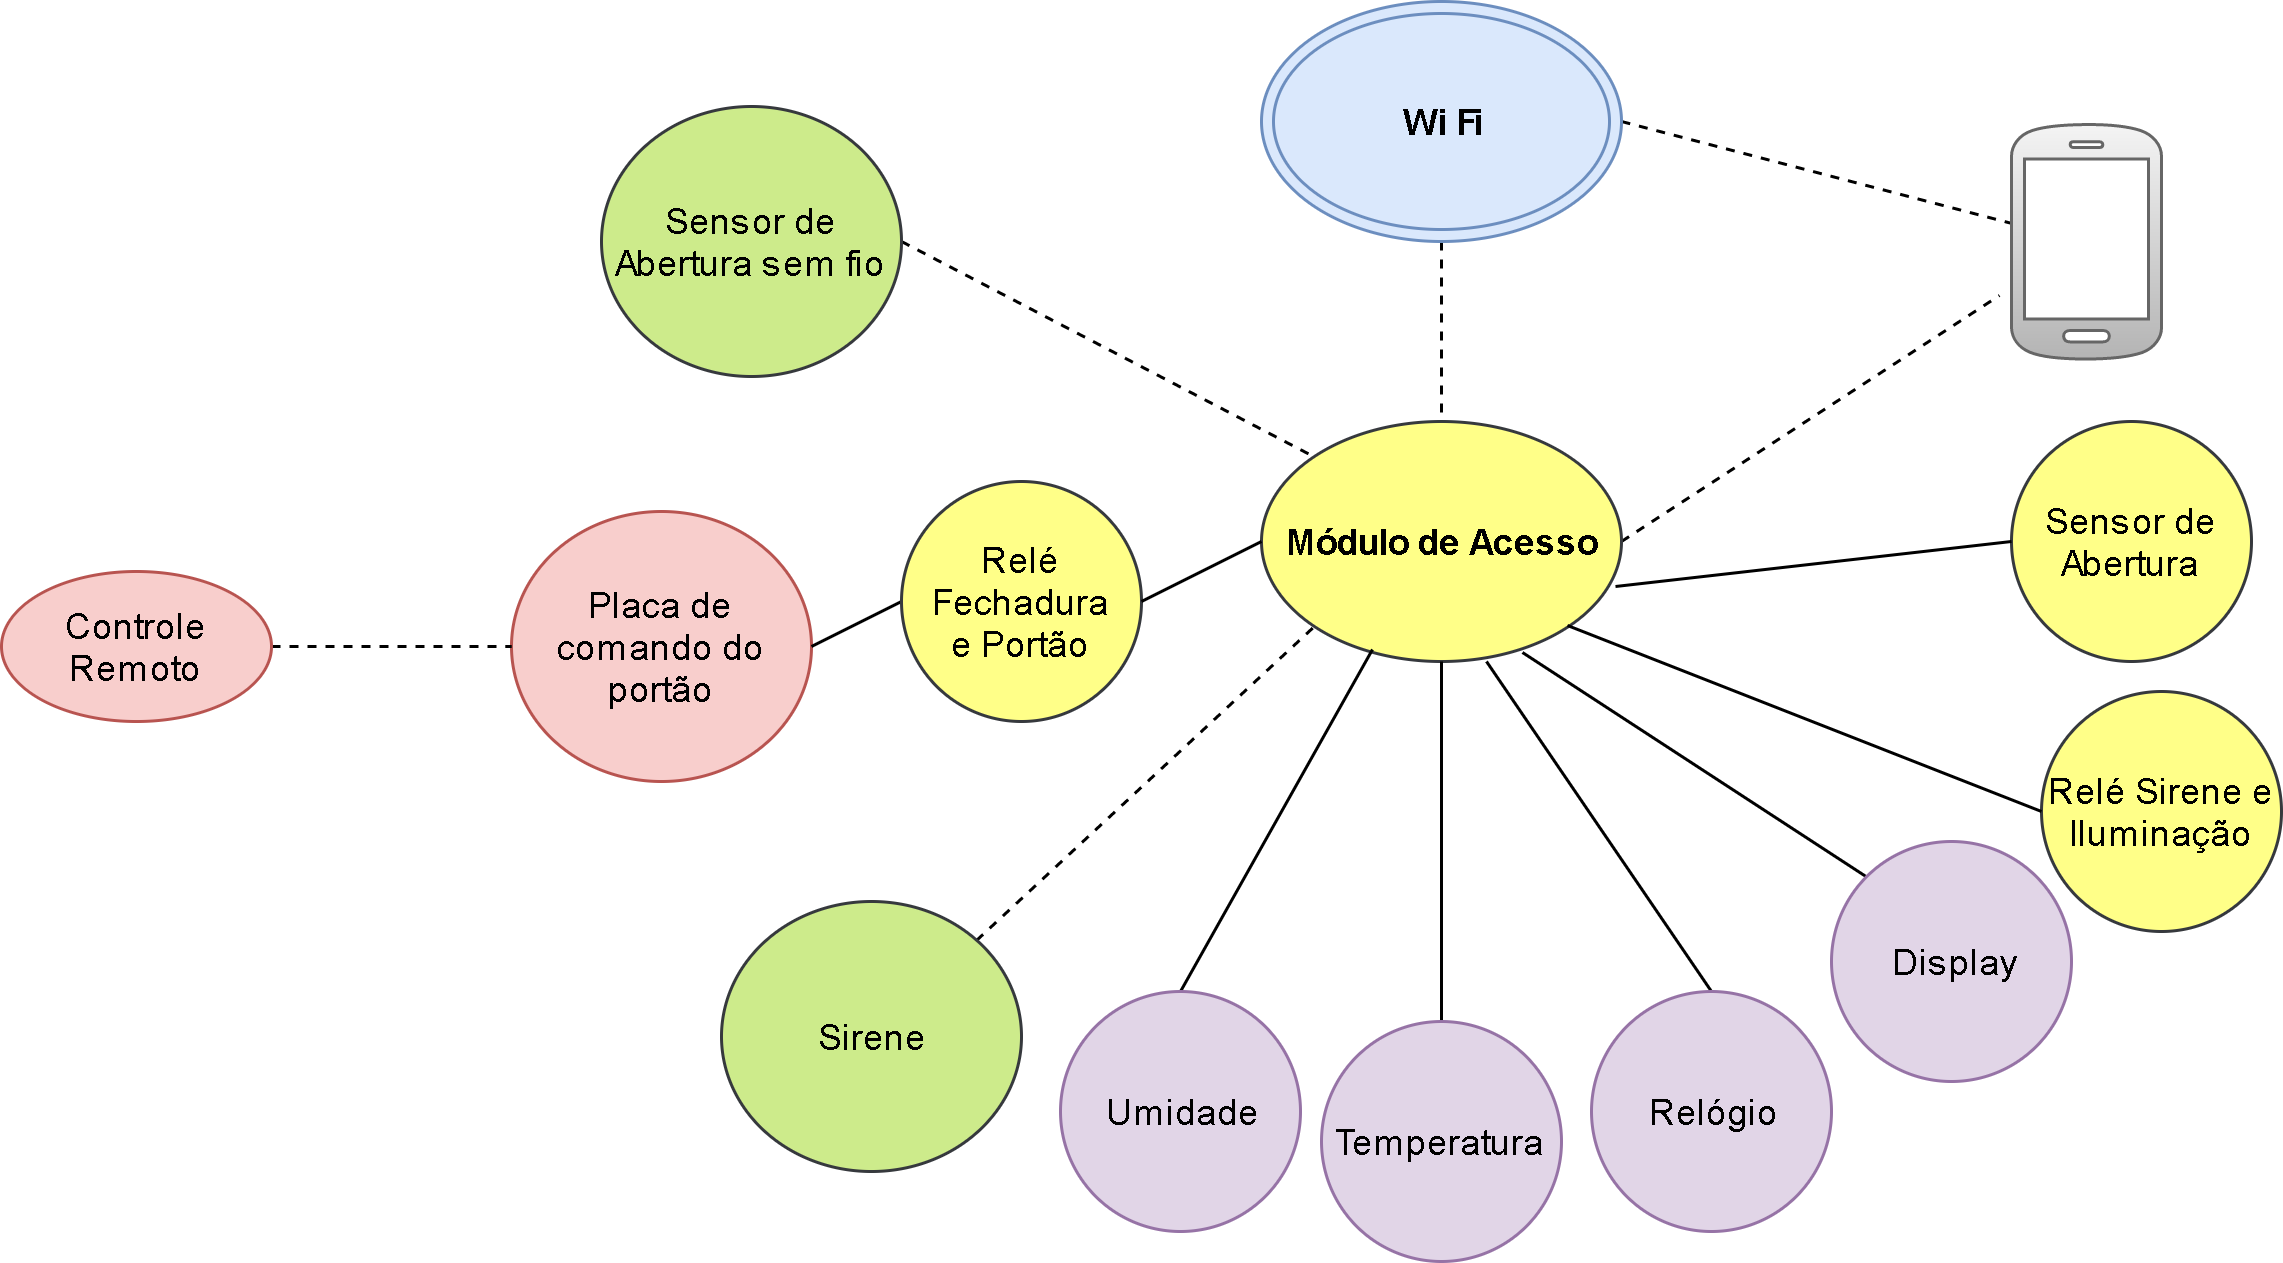
\includegraphics[width=0.8\textwidth]{diagramaModuloAcesso}
\label{fig:diagramaModuloAcesso}
\end{figure}

A Figura \ref{fig:diagramaModuloAcesso} ilustra em vermelho dispositivos já existentes no mercado, como o controle remoto. O sensor e a sirene sem fio adicionais são mostrados em verde --- são dispositivos externos ao módulo, que se comunicam por ondas de rádio. O próprio módulo de acesso, com um \emph{buzzer} embutido, e sua conexão com a rede local Wi-Fi ou sua conexão direta com o celular (quando o módulo opera como um ponto de acesso de rede) estão em amarelo. As funcionalidades adicionais são marcadas em roxo.

A comodidade, no exemplo em questão, está em abrir o portão por meio do celular, ao utilizar o aplicativo web ou o aplicativo local de emergência, sem a necessidade de carregar uma chave ou controle.

Entretanto, é necessário que a realização do controle de acesso seja feita de maneira segura. Assim, é empregado um algoritmo de rotação de teclas, para evitar que pessoas mal-intencionadas possam:

\begin{enumerate}
	\item Olhar e copiar a senha que o usuário digita em seu celular;
	\item \label{alt:manInTheMiddle} Copiar os dados de abertura e usá-los mais tarde (\textit{middle man}).
\end{enumerate}

Na alternativa alternativa \ref{alt:manInTheMiddle}, a cada acesso, um novo mapeamento de teclas é gerado e enviado ao usuário. Mesmo que haja cópia das credenciais, ela não funcionará devido ao mapeamento ter mudado. Observe ainda que a fechadura eletrônica, por si só, já estava vulnerável a este tipo de ataque --- há, inclusive, dispositivos copiadores de senhas comercializados.

Outro aspecto de segurança é a preocupação dos usuários em esquecer a porta ou portão abertos. Para mitigar esse perigo, o módulo deve monitorar por meio de um sensor o estado vigente (aberto ou fechado) conforme o requisito RF-1, e alertar localmente (por meio de \textit{buzzer}) e remotamente (e.g. por email ou notificação no smartphone) o usuário conforme o requisito RF-2. Essa e outras configurações como a de rede são acessadas por uma senha diferente daquela de abertura, de modo que a interface básica seja simples para uso.

Para o caso de falha de envio de notificação (e.g. servidor fora do ar ou indisponibilidade na conexão), há um algoritmo de novas tentativas com tempos progressivamente maiores conforme as falhas ocorrerem, buscando deixar o módulo disponível para outras funções. Tratamento análogo é realizado no servidor local, e no sistema de mensageria, de modo a evitar perdas de mensagens mesmo em situações desfavoráveis. Para o caso de falta de conexão à Internet, o módulo não seria controlável pela nuvem com o aplicativo web, mas sim com o aplicativo emergencial usando a ativação do \textit{Access Point}, desenvolvido para operar diretamente com os módulos, sem intermédio do servidor local e dos serviços remotos.

Por meio das credenciais disponíveis no sistema, é possível saber qual dos usuários solicitou a abertura do portão. A persistência destes acessos pode ser analisada e, utilizando-se técnicas de aprendizado de máquina, perfis de acesso podem ser determinados, e evoluir até que o sistema saiba quando houver um acesso em horário inesperado e possa notificar o usuário remotamente, conforme o requisito RF-5. O aprendizado de máquina é fundamental aqui para descobrir comportamentos que podem ser entendidos como suspeitos. Um exemplo prático de caso de uso seria um usuário que costuma chegar em um horário semelhante todos os dias e realizar certo conjunto de tarefas na casa. Uma tentativa de acesso que não se enquadre em tais padrões pode ser produto de atividade suspeita, a qual pode ser informada pela casa para uma central, que acionaria a polícia caso seja confirmado que não se trata de um falso positivo.

\subsection{Módulo de Quarto/Sala/Cozinha}
Um dos módulos com muitas opções de implementação e uso é o módulo de quarto, pois ele também pode ser usado no controle de iluminação para corredores, salas e ambientes externos.

\begin{figure}[H]
	\centering
	\caption{Diagrama ilustrativo do Módulo de Quarto/Sala/Cozinha}
	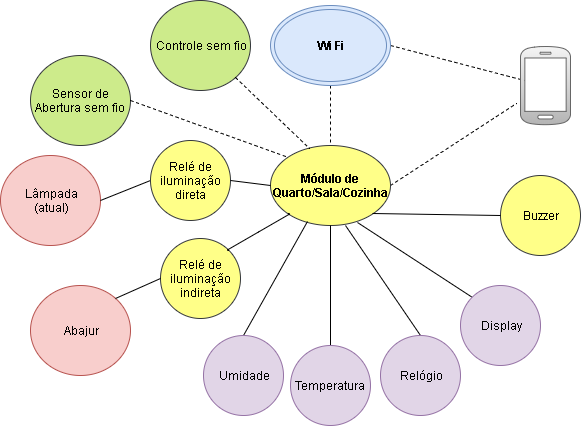
\includegraphics[width=0.8\textwidth]{diagramaModuloQuarto}
	\label{fig:diagramaModuloQuarto}
\end{figure}

O diagrama ilustra equipamentos externos ao sistema (lâmpada e abajur) em vermelho, enquanto o controle e sensor de abertura possuem comunicação sem fio. Em roxo, representam-se os equipamentos opcionais.

Como principais funcionalidades, tem-se o despertador (configurado pelo usuário, que também pode receber recomendações baseadas na informação gerada pelo monitoramento de seus ciclos de sono); monitoramento de temperatura e umidade do ambiente (que podem ser notificadas ao usuário, caso informem valores fora de determinados intervalos); controle de iluminação (da luz direta, que é a lâmpada central do ambiente, com maior potência, e da luz indireta, que é usualmente um abajur ou uma lâmpada com menor potência, usada para leitura); e estado da janela, para verificar remotamente se a janela está fechada ou não (por notificação ou visualização no aplicativo, útil para dias chuvosos). Além disso, se o módulo for instalado em ambientes internos e externos, o usuário pode usufruir de dados de temperatura e umidade, que podem ser usados para escolher a vestimenta, optar por levar guarda-chuva na ida para o trabalho ou decidir se é mais vantajoso deixar roupas secando dentro ou fora de casa, e em que períodos.

O módulo de quarto pode ser acoplado ao sistema existente --- fisicamente, é instalado no mesmo lugar do interruptor ---, e possui estados para o despertador. No estado inicial, somente a luz indireta é ligada. Após determinado tempo programável pelo usuário, há avisos sonoros periódicos. No terceiro estado, os períodos são menores. Finalmente, no quarto estado a luz direta é ligada e os avisos sonoros são ininterruptos. Até o terceiro estado, o alarme pode ser desarmado (apertar duas vezes) ou entrar em estado soneca (apertar única vez) diretamente no módulo. Já no estado 4, a critério anterior do usuário, o alarme pode ser desarmado somente fisicamente em outro módulo presente em um segundo aposento --- por exemplo, na sala. Esse módulo pode variar de dia para dia, caso o usuário assim desejar. O sistema desarma o alarme após 40 minutos.

O display possui iluminação automática por meio de circuito baseado em LDR para não apresentar brilho muito intenso quando todas as luzes estiverem desligadas. Para o controle da iluminação, há diferentes tempos de desligamento. Por exemplo, quando ocorre controle manual pelo botão presente no módulo, o tempo pode ser maior (e.g. 30 minutos). Já pelo modo automático, quando a luz já foi ligada pelo próprio módulo, o tempo para desligamento pode ser menor (e.g. 4 minutos).

Com o monitoramento da presença, há um reinício da contagem para desligamento sempre que houver presença detectada, de forma a inibir acionamentos desnecessários do relé. Outra aplicação para o monitoramento da presença é a descoberta de comportamento anormal. Por exemplo, se o usuário sempre toma café entre 8 e 10 horas, e não apresentar presença na casa até às 15 horas, o sistema pode notificar emails de parentes cadastrados.

\subsection{Módulo de Aquário}

Devido a altos custos de compra, implantação e manutenção de um aquário, que pode ser de água doce ou salgada, e até abrigar espécies raras, é desejável que uma série de riscos sejam mitigados. Dentre tais riscos, destacam-se:

\begin{table}[hbp]
		\centering
		\caption{Riscos para o aquário}
		\resizebox{\textwidth}{!}{%
		\begin{tabular}{cp{8cm}p{8cm}}
			\toprule
			\textbf{Perigo/Necessidade} 					& \textbf{Origem} 																			& \textbf{Consequência}  \\
			\midrule
			Aquecimento acidental 							& Ajuste errado da temperatura do termostato												& Superaquecimento; risco de mortes (peixes e plantas) \\
			Falta de água 									& Vazamento ou evaporação natural															& Mal funcionamento ou queima da bomba submersa (à longo prazo, falta de oxigenação da água) \\
			Falta de circulação de água 					& Entupimento do tubo de circulação ou mal funcionamento da bomba							& Falta de oxigenação da água, ocasionando em risco de mortes (peixes) \\
			Iluminação adequada								& Existência de plantas e/ou iluminação natural insuficiente no ambiente do aquário			& Ambiente nocivo para os peixes, risco de morte das plantas (principalmente durante períodos de esquecimento/viagens) \\
			\bottomrule
	\end{tabular}}
	\label{table:riscosaquario}
\end{table}

Sobre o caso específico da residência onde foram executados os testes de campo, considere um aquário com 50 litros de água, com uma bomba para circulação de água e um aquecedor, com cerca de 50 peixes de pequeno porte, que são sensíveis à variação brusca de temperatura.

Na ocasião de troca de água do aquário, cerca de 20\% do volume total é substituído. A saída de água se dá por um funil, e a adição é realizada pela bomba, que introduz água limpa, sem cloro e com menos amônia e outros compostos nocivos aos peixes (que justificam essa troca periódica de água). O monitoramento do nível da água pode também mitigar o risco de esquecimento.

\begin{figure}[H]
	\centering
	\caption{Diagrama ilustrativo do Módulo de Aquário}
	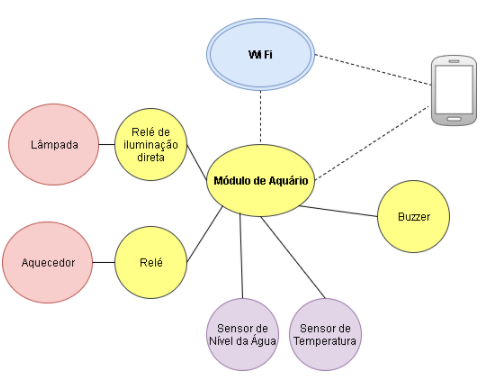
\includegraphics[width=0.8\textwidth]{diagramaAquario}
	\label{fig:diagramaAquario}
\end{figure}

Para mitigar os riscos descritos anteriormente, foi desenvolvido o módulo de aquário, que permite:

\begin{enumerate}
	\item Controle de horários em que a lâmpada fica acesa, fornecendo uma iluminação adequada para as plantas e peixes do aquário em períodos curtos de viagem;
	\item Monitoramento do nível de água do aquário principal, com disparo de alerta pelo aplicativo quando não estiver no nível esperado --- o que pode ocorrer por muita evaporação, vazamento ou problema com a bomba;
	\item Monitoramento da temperatura do aquário, e bloqueamento do aquecedor caso a água já esteja numa temperatura desejável, evitando superaquecimento devido a mal funcionamento do termostato --- isso é feito por meio de ligação em série com o termostato do aquário;
	\item Nos casos de perigo acima descritos, também disparar alerta sonoro localmente por meio do \emph{buzzer}.

\end{enumerate}

\subsection{Módulo de Interface com Sistema de Alarmes}

O módulo de interface com o sistema de alarmes monitora dois aspectos específicos: um relativo à presença, possuindo sensores no corredor e na sala da residência, e outro relativo à porta da sala, com um sensor único na porta da residência. O módulo implementado foi instalado em uma residência em Jarinu - SP.

\begin{figure}[H]
	\centering
	\caption{Diagrama ilustrativo do Módulo de Interface com Sistema de Alarmes}
	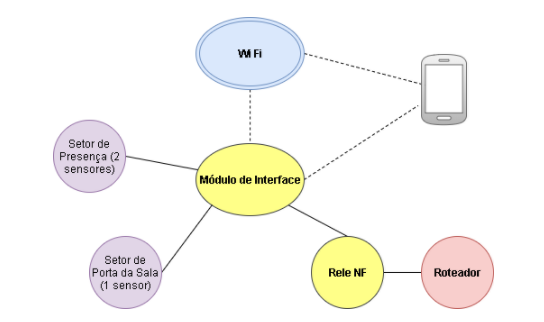
\includegraphics[width=0.8\textwidth]{diagramaAlarme}
	\label{fig:diagramaAlarme}
\end{figure}

Um problema recorrente é a conexão com a Internet, que, apesar da indicação de estado válido e conectado, não fornecia acesso a sites, tampouco acesso externo por meio de abertura de porta no roteador. Para contornar esse problema e permitir que o módulo esteja disponível para coleta de dados e persistência em cartão SD, foi instalado também um relé NF (normalmente fechado) em série com a alimentação do roteador (no caso do módulo estar desligado, o roteador ficará ligado).

Já quando há erro persistente (maior que 10 vezes em intervalos de 2 a 3 minutos) ao realizar a operação de \emph{ping} com sites ou servidores conhecidos, o módulo reinicia a conexão atuando diretamente no roteador. Ocorre a execução deste procedimento em intervalos cada vez mais espaçados, de forma a não executar muitas vezes o reinício do roteador sem que a conexão seja reestabelecida com sucesso. Nas primeiras tentativas, tem-se um intervalo de 3 minutos até a nova tentativa, a partir da terceira vez um intervalo de 10 minutos, e assim por diante, até um máximo de 30 minutos.

Outra dificuldade encontrada em sua instalação em campo foi a obtenção de endereço IP dinâmico em uma rede em que outros dispositivos, tais como celulares e tablets, também obtinham endereços IP dinâmicos, gerando indisponibilidades do módulo. Com a mudança do endereço IP para fixo, em outro intervalo de endereçamento, o módulo passou a ter alta disponibilidade, ficando até semanas sem reiniciar.
